Dans cette exercice nous faisons appel à une fonction annexe pour récupérer la fonction échelon.

Cette fonction prend en paramètre le vecteur représentant l'intervalle de visualisation ainsi que le décalage que l'on souhaite appliquer à l'échelon.

La courbe ci dessous nous illustre le filtre discret que nous avons à disposition :

\begin{figure}[H]
\centering
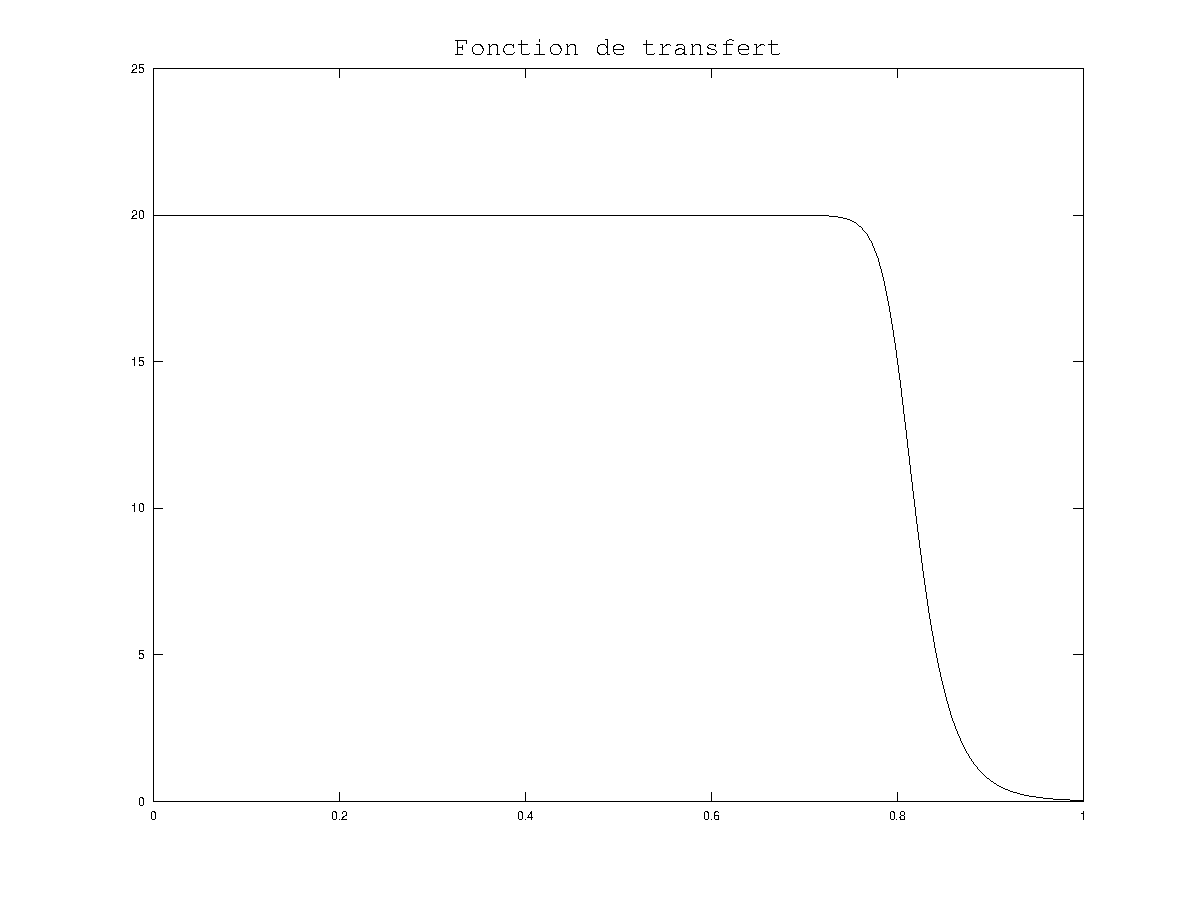
\includegraphics[width=9cm]{resEx2/fctTransfert.pdf}
\caption{Fonction de transfert du filtre $2*sin(\frac{n*\pi}{2})[u(n+3)-u(n-4)]$}
\end{figure}

Le signal d'entrée définit par la fonction $\frac{n}{2}[u(n)-u(n-6)]$ est le suivant:

\begin{figure}[H]
\centering
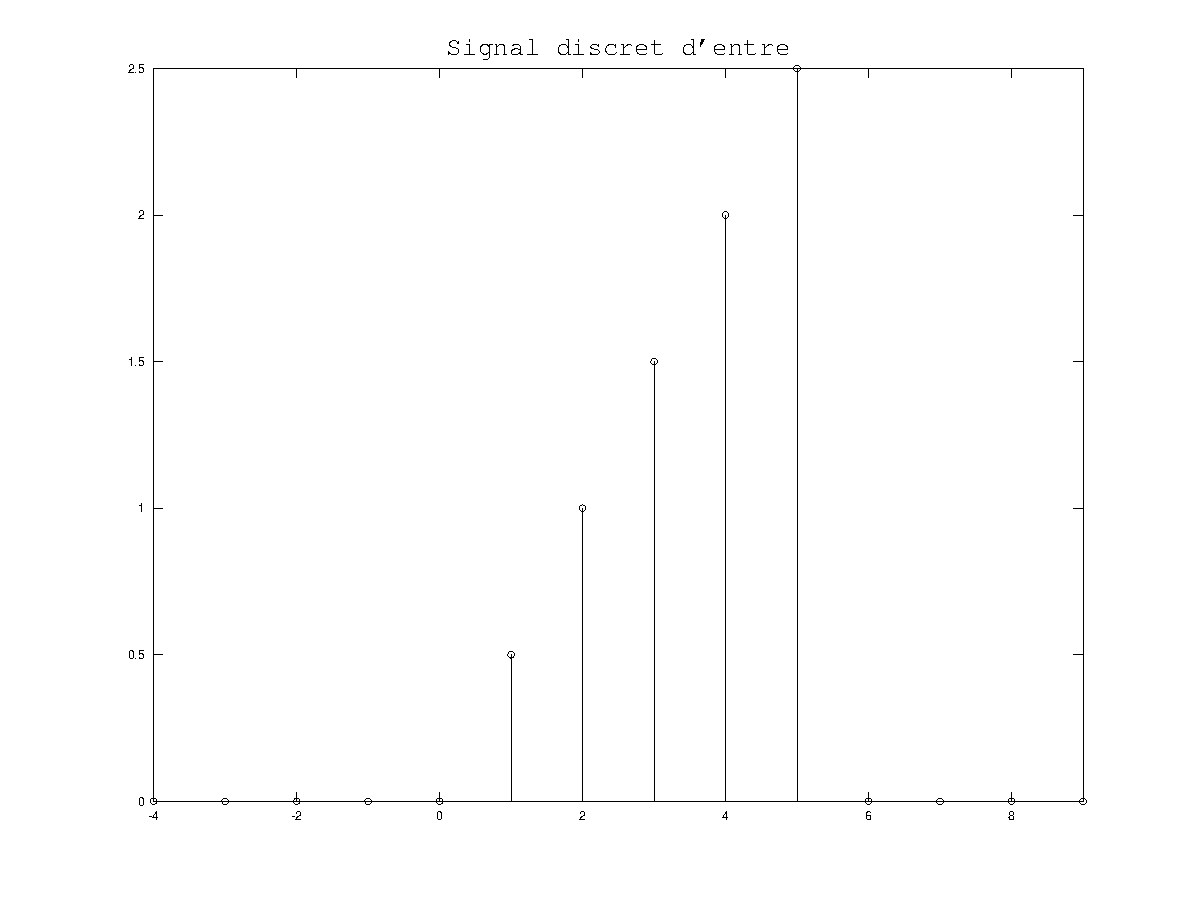
\includegraphics[width=9cm]{resEx2/signalEntree.pdf}
\caption{Signal d'entrée}
\end{figure}

La réponse impulsion du filtre précédent nous donne la figure suivante : 

\begin{figure}[H]
\centering
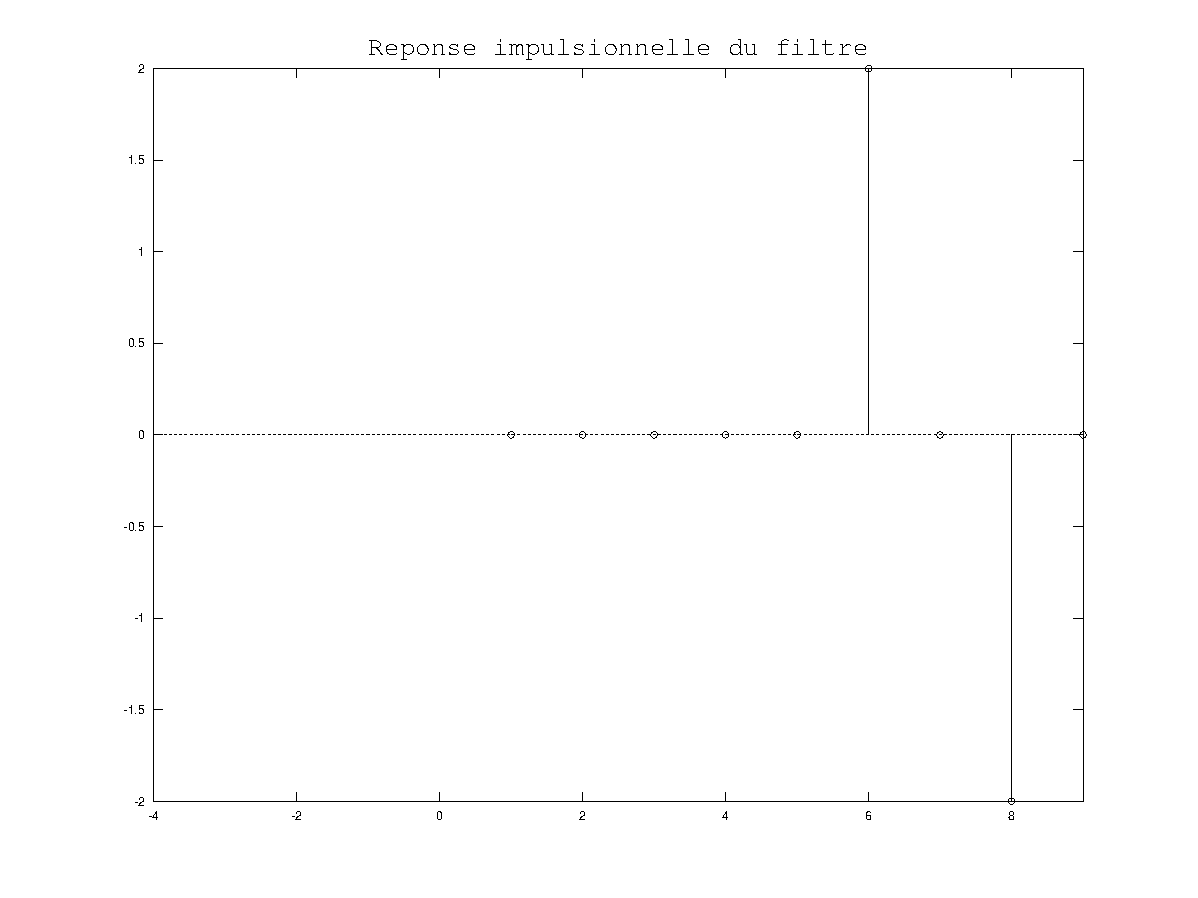
\includegraphics[width=9cm]{resEx2/repImpulsionnelle.pdf}
\caption{Réponse impulsionnelle du filtre}
\end{figure}

Le produit de convolution du filtre et du signal nous donne le signal ci dessous :

\begin{figure}[H]
\centering
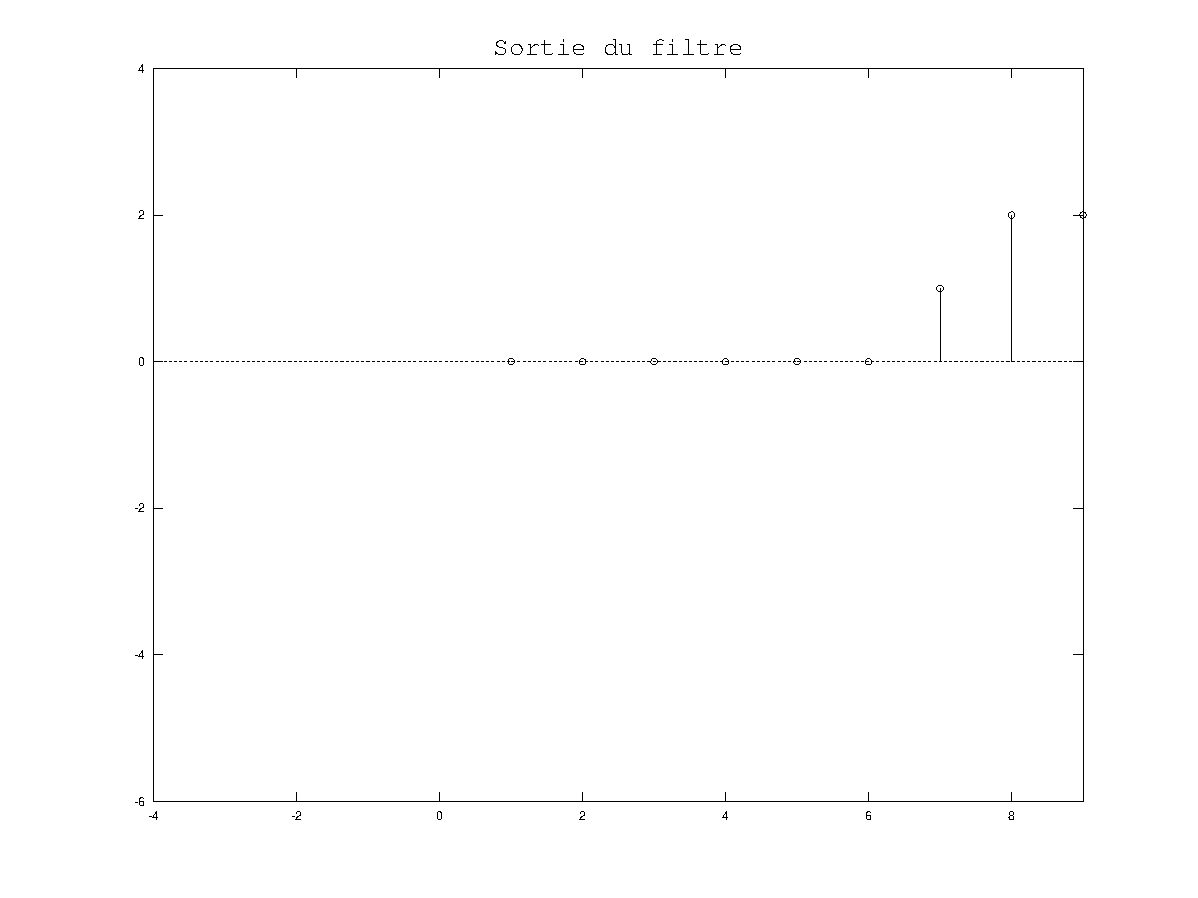
\includegraphics[width=9cm]{resEx2/sortieFiltre.pdf}
\caption{Signal en sortie du filtre}
\end{figure}
